\subsection{Model Development}

Developing a neural net isn't just about figuring out the neurons for the network and adjusting the weights.
The task of making a neural net can be broken up into 3 main parts.

\begin{figure}[H]
\centering
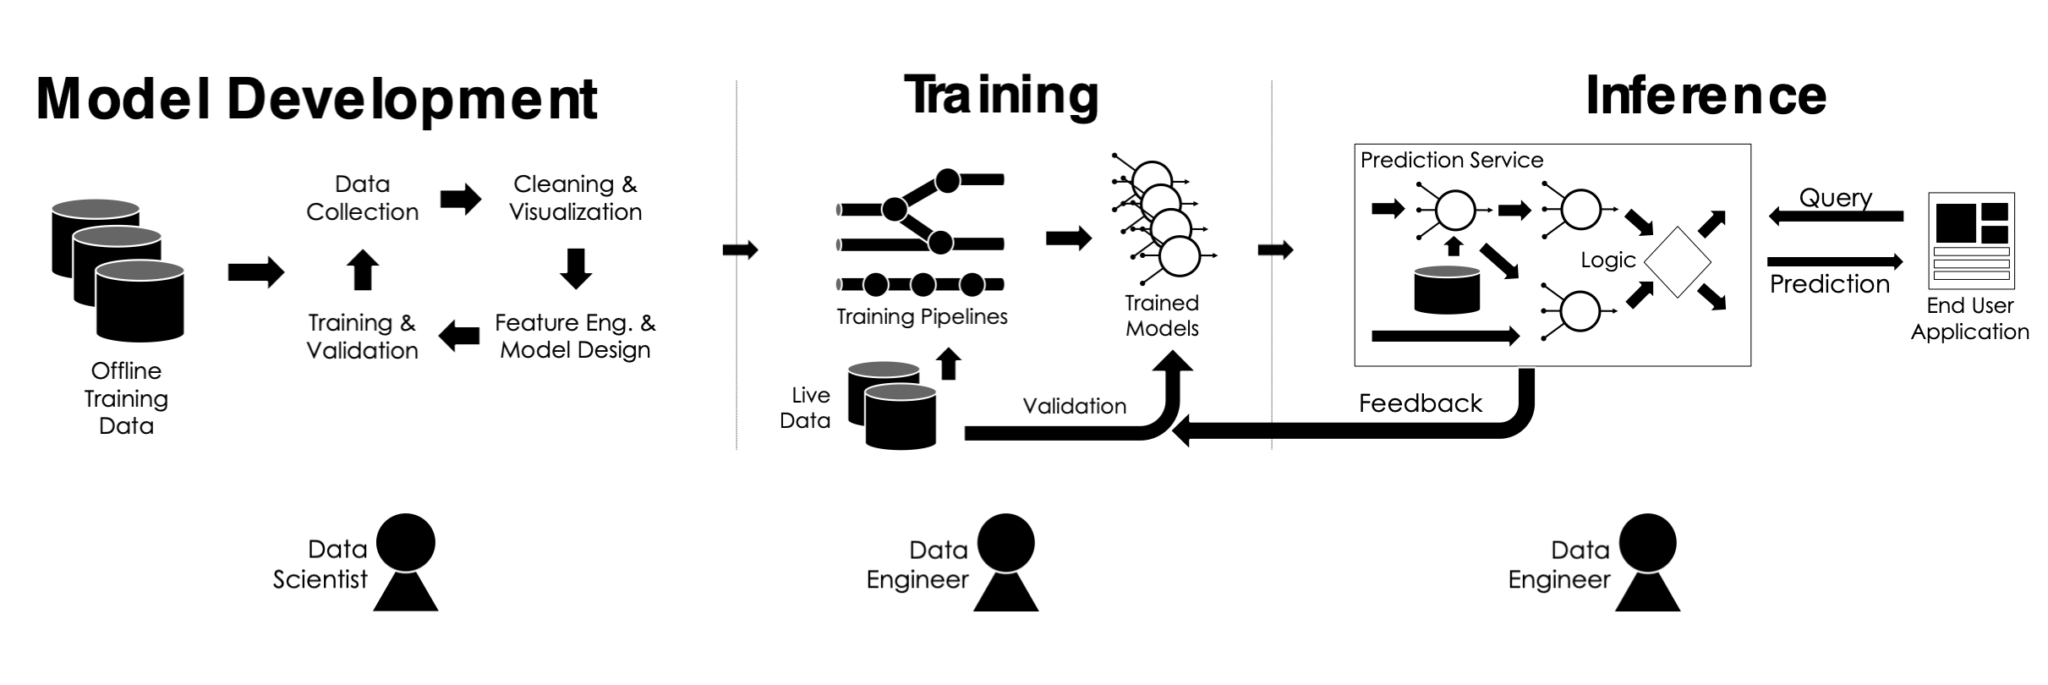
\includegraphics[width=120mm]{figures/mlLifecycle.png}
\caption{Model development \cite{Yang_2020}}
\label{lifecycle}
\end{figure}

The first step of any kind of model development is looking at both what kind of data is available as well as what kind of input we might want to make on the model.
The data may be scattered about in many places and often will require processing before it can be vectorized.

In the context of neutrino reconstruction, this may require running monte carlo simulations with standard software e.g. (LArSoft, NDsim) and then taking the output from those simulations, processing it into standard images that libraries like pytorch or tensorflow can take as input.
It is also important to think about standardizing the size of those images and thinking about how to toss out the sheer amount of data that has no hits in it because neutrino events are so sparse.

Once that has been done, we can look at actually implementing a neural network based on that data.
This involves setting out training pipelines which will determine how the data flows, as well as figuring out the structure of the network that will be made.
Tests also have to be written for the network so that it can be deployed robustly.
Once the training with the training dataset is complete, the model has to be validated with a validation dataset.
The validation set will also be a set where the answers are previously known so we can see how well the model performs on data that it hasn't previously been run on.

Once the model has been validated, it can finally be deployed for real world data where we don't have the answers.
This is the inference part of the model lifecycle \cite{Zell_1997}.

